% ============================================================
%  A Comparison of Selected Organic Materials for
%  Low Orbiting Spacecraft Hull Plating
%  Compiler: XeLaTeX  (requires Cambria and Times New Roman)
% ============================================================
\documentclass[11pt,a4paper]{article}

% ── packages ────────────────────────────────────────────────
\usepackage{fontspec}
\usepackage{geometry}
\usepackage{titlesec}
\usepackage{setspace}
\usepackage{graphicx}
\usepackage{booktabs}
\usepackage{array}
\usepackage{tabularx}
\usepackage{caption}
\usepackage{amsmath}
\usepackage{amssymb}
\usepackage{indentfirst}
\usepackage{enumitem}
\usepackage{multirow}
\usepackage{xcolor}
\usepackage[english]{babel}
\usepackage{url}
\usepackage{longtable}

% ── fonts ────────────────────────────────────────────────────
\setmainfont{Times New Roman}
\newfontfamily\cambriafont{Cambria}

% ── page geometry (top 2.5 cm, bottom 7 cm, L/R 4 cm) ──────
\geometry{
  a4paper,
  top    = 2.5cm,
  bottom = 7.0cm,
  left   = 4.0cm,
  right  = 4.0cm
}

% ── paragraph / line spacing ────────────────────────────────
\setlength{\parindent}{0.5cm}
\setlength{\parskip}{0pt}
\linespread{1.0}

% ── section formatting ───────────────────────────────────────
% Introduction / main sections: TNR 12pt bold, before 24pt, after 6pt
\titleformat{\section}[block]
  {\fontsize{12}{14.4}\selectfont\bfseries}
  {}{0em}{}
\titlespacing*{\section}{0pt}{24pt}{6pt}

% Main subheadings: TNR 12pt bold, before 16pt, after 5pt
\titleformat{\subsection}[block]
  {\fontsize{12}{14.4}\selectfont\bfseries}
  {}{0em}{}
\titlespacing*{\subsection}{0pt}{16pt}{5pt}

% Second-level subheadings: TNR 11pt bold, before 16pt, after 6pt
\titleformat{\subsubsection}[block]
  {\fontsize{11}{13.2}\selectfont\bfseries}
  {}{0em}{}
\titlespacing*{\subsubsection}{0pt}{16pt}{6pt}

% Summary / References headers: TNR 12pt bold, before 18pt, after 6pt
\newcommand{\specialsection}[1]{%
  \vspace{18pt}%
  {\fontsize{12}{14.4}\selectfont\bfseries #1\par}%
  \vspace{6pt}%
}

% ── figure / table captions ──────────────────────────────────
% Figure caption: 10pt italic bold, below figure, before/after 6pt
\captionsetup[figure]{
  labelfont  = {bf,it,footnotesize},
  textfont   = {bf,it,footnotesize},
  labelsep   = period,
  justification = justified,
  singlelinecheck = false,
  aboveskip  = 6pt,
  belowskip  = 6pt
}
% Table caption: 10pt italic bold, ABOVE table, before/after 6pt
\captionsetup[table]{
  labelfont  = {bf,it,footnotesize},
  textfont   = {bf,it,footnotesize},
  labelsep   = period,
  justification = justified,
  singlelinecheck = false,
  aboveskip  = 6pt,
  belowskip  = 0pt,
  position   = above
}

% ── footnotes ────────────────────────────────────────────────
\renewcommand{\footnotesize}{\fontsize{9}{10.8}\selectfont}

% ── graphics path ────────────────────────────────────────────
\graphicspath{{../raport_zbiorczy/plots/}}

% ============================================================
\begin{document}
\pagestyle{plain}

% ────────────────────────────────────────────────────────────
%  TITLE BLOCK
% ────────────────────────────────────────────────────────────
\begin{center}
  {\cambriafont\fontsize{14}{16.8}\selectfont\bfseries
    A Comparison of Selected Organic Materials\\[4pt]
    for Low Orbiting Spacecraft Hull Plating\par}

  \vspace{12pt}

  {\cambriafont\fontsize{10}{12}\selectfont\bfseries
    Kalina Banaszek, Magdalena Dzięgiel, Filip Zdrojewski\par}

  \vspace{5pt}

  {\fontsize{9}{10.8}\selectfont
    AGH University of Krakow\\
    Faculty of Mechanical Engineering and Robotics\par}
\end{center}

\vspace{8pt}

% ────────────────────────────────────────────────────────────
%  ABSTRACT (English)
% ────────────────────────────────────────────────────────────
\begingroup
  \setlength{\leftskip}{0.75cm}
  \setlength{\rightskip}{0.75cm}
  \fontsize{9}{10.8}\selectfont\noindent
  \textbf{Abstract:}
  Spacecraft operating in low Earth orbit (LEO) and during the launch phase are
  exposed to simultaneous extreme threats: atomic oxygen~(AO) erosion, ultraviolet
  radiation, thermal cycling between $-150\,^{\circ}$C and $+150\,^{\circ}$C,
  micrometeoroid and orbital debris~(MMOD) impacts, and heat fluxes of
  1--10\,MW/m$^{2}$ during ascent. The selection of hull plating and thermal
  protection system (TPS) materials requires balancing low areal density, high
  structural strength, thermal stability, and surface durability.
  This paper presents a systematic comparison of thirteen organic materials
  (M1--M13) covering polyimide films, thermoset resins, elastomers, aramid
  fibres, and advanced composites. Mechanical and thermal properties at room
  temperature and as a function of temperature were compiled from manufacturer
  datasheets and peer-reviewed literature. Comparison charts and a five-criterion
  scoring methodology identify the top five candidate materials: Kapton~HN~(M1)
  and POSS-polyimide~(M2) for LEO surface films; Kevlar-29/49~(M7) for
  structural and Whipple-shield applications; carbon-fibre/phenolic
  composite~(M12) for high-heat-load TPS; and polysiloxane composite~(M6) as
  a versatile ablative-structural hybrid.
  \par\vspace{4pt}
  \noindent\textbf{Keywords:}
  ablative materials, atomic oxygen, aramid fibres, Kapton, Kevlar,
  low Earth orbit, organic composites, polyimide,
  spacecraft, thermal protection system
\endgroup

\vspace{10pt}

% ────────────────────────────────────────────────────────────
%  1. INTRODUCTION
% ────────────────────────────────────────────────────────────
\section*{Introduction}

The protective plating of a spacecraft must satisfy radically different
requirements during two successive mission phases. During launch and ascent, the
vehicle is exposed to aerodynamic heat fluxes reaching 1--10\,MW/m$^{2}$,
acoustic loads up to 160\,dB, and structural accelerations of 5--12\,$g$
(Natali et al.\ 2012, p.\,1). Once in low Earth orbit at altitudes of 160--2000\,km,
the dominant threats change to atomic oxygen at fluences of
$10^{20}$--$10^{21}$\,atoms/cm$^{2}$ per year, vacuum-ultraviolet radiation, and
thermal cycling between $-150\,^{\circ}$C and $+150\,^{\circ}$C with a period
of approximately 90\,minutes (Gouzman et al.\ 2010, p.\,2438).

Organic materials occupy a strategic position in spacecraft design because
they can be tailored through polymer chemistry and fibre reinforcement to address
several of these requirements simultaneously at low areal density. Polyimide films
provide radiation resistance, dimensional stability, and a wide service
temperature range, making them the standard material for multi-layer insulation
(MLI) blankets. Aramid fibres deliver specific tensile strengths exceeding
2.0\,km$^{2}$/s$^{2}$, enabling lightweight Whipple shields and pressure vessels.
Ablative composites pyrolyse controllably, consuming heat through endothermic
reactions and leaving a protective char layer.

This paper compiles and analyses the key mechanical and thermal properties of
thirteen organic materials selected on the basis of current or prospective use in
spacecraft hulls and TPS. Materials are labelled M1--M13. The objective is to
provide a single reference document that facilitates rational material selection
for specific sub-systems, supported by temperature-dependent data covering the
full LEO thermal envelope.

% ────────────────────────────────────────────────────────────
%  2. ENVIRONMENTAL CONDITIONS
% ────────────────────────────────────────────────────────────
\section*{Environmental Conditions}

The design envelope for spacecraft hull materials is defined by two overlapping
phases summarised in Table~1.

\begin{table}[h!]
\centering
\caption{\textit{Design conditions for spacecraft hull materials during launch
  and LEO service.}}
\label{tab:environments}
\vspace{4pt}
\begin{tabular}{p{2.2cm} p{3.8cm} p{4.5cm}}
\toprule
\textbf{Phase} & \textbf{Primary threats} & \textbf{Key material requirements} \\
\midrule
Launch / ascent
  & Heat flux 1--10\,MW/m$^{2}$;\newline vibration; acceleration 5--12\,$g$
  & Ablation / TPS;\newline high mechanical strength;\newline low areal density \\
\addlinespace[4pt]
LEO (orbit)
  & AO $10^{20}$--$10^{21}$\,at/cm$^{2}$/yr; UV; thermal cycling
    $-150$ to $+150\,^{\circ}$C; MMOD
  & AO/UV resistance;\newline dimensional stability;\newline $K_{\mathrm{IC}} > 1\,\mathrm{MPa\,m}^{0.5}$ \\
\bottomrule
\end{tabular}
\end{table}

Atomic oxygen is the dominant chemical threat below 600\,km altitude. It erodes
most organic polymers at rates of $10^{-24}$--$10^{-23}$\,cm$^{3}$/atom.
Kapton erodes at approximately $3 \times 10^{-24}$\,cm$^{3}$/atom; aliphatic
polymers such as UHMWPE erode 3--5 times faster due to the absence of aromatic
rings in the backbone. POSS-modified polyimides and polysiloxane composites
benefit from passive self-passivation: AO oxidises surface silicon atoms to
SiO$_{2}$, forming a self-healing ceramic barrier (Gouzman et al.\ 2010, p.\,2440).

Thermal cycling introduces cyclic mechanical strains proportional to the
coefficient of thermal expansion (CTE) mismatch between bonded layers. For a
polymer film adhered to a metallic structure, strains per cycle can reach
0.1--0.5\%, requiring high fatigue resistance and fracture toughness.

% ────────────────────────────────────────────────────────────
%  3. MATERIALS
% ────────────────────────────────────────────────────────────
\section*{Materials}

\subsection*{Polyimide Films}

\textbf{Kapton HN (M1)} is a poly(4,4$'$-oxydiphenylene-pyromellitimide) film
produced by DuPont and used on spacecraft since the Apollo programme. Its room-temperature
tensile strength (UTS) of 231\,MPa at a density of 1420\,kg/m$^{3}$ gives a
specific strength of 163\,kN$\cdot$m/kg. Young's modulus is 2.5\,GPa and
fracture toughness is 1.65--5.4\,MPa$\,\mathrm{m}^{0.5}$ depending on film
thickness and orientation (DuPont 2023). The continuous service range of
$-269$ to $+400\,^{\circ}$C covers both cryogenic propellant tanks and
aerodynamic heating. Thermal conductivity is 0.12\,W/(m$\cdot$K). The principal
LEO limitation is AO erosion, which requires a protective SiO$_{2}$ or Al
coating on sun-facing surfaces.

\textbf{POSS-Polyimide (M2)} incorporates polyhedral oligomeric silsesquioxane
(POSS) nanocages into the polyimide backbone. AO oxidises the surface Si atoms
to SiO$_{2}$, forming a self-passivating ceramic layer that suppresses further
erosion — the key advantage over Kapton for long-duration LEO missions. UTS is
approximately 210\,MPa, $E = 2.3\,\mathrm{GPa}$, and operating range is
$-269$ to $+450\,^{\circ}$C (Brunsvold et al.\ 2004, p.\,303;
Gouzman et al.\ 2010, p.\,2439).

\subsection*{Thermoset Resins}

\textbf{Phenol-Formaldehyde Resin (M3a)} — phenol-formaldehyde thermosetting resins have been
the matrix material of choice for ablative TPS since the 1960s. Neat resin has
UTS = 45\,MPa, $E$ = 3.5\,GPa, and a brittle failure mode (elongation~1\%). At
temperatures above 300\,°C the resin pyrolyses, forming a porous char with
approximately 55\% carbon yield, which insulates the underlying structure. The
maximum effective ablative protection temperature exceeds 2000\,°C
(Natali et al.\ 2012, p.\,3). Density is 1250\,kg/m$^{3}$.

\textbf{Phthalonitrile Resin (M4)} represents the next generation of
high-temperature thermosets. Cure proceeds without volatile byproducts,
yielding void-free, low-outgassing parts — a critical requirement near spacecraft
optics and sensors. The glass transition temperature $T_{\mathrm{g}}$ exceeds
375\,°C, the highest continuous service temperature of any unreinforced polymer
in this study. UTS = 65\,MPa, $E$ = 4.0\,GPa; char yield is approximately 65\%
(Hergenrother et al.\ 2005, p.\,7853; Laskoski et al.\ 2006, p.\,4559).

\subsection*{Elastomers and Composite Films}

\textbf{RTV Silicone (M5)} — room-temperature-vulcanising polydimethylsiloxane
elastomers (e.g.\ Momentive RTV566) are used as structural adhesives, sealants,
and vibration dampers in satellite assemblies. UTS is only 6\,MPa but elongation
reaches 400\%, giving a uniquely hyperelastic stress--strain response. The
service range is $-115$ to $+300\,^{\circ}$C; at cryogenic temperatures Young's
modulus rises sharply from 3\,MPa at room temperature to approximately
2000\,MPa at $-115\,^{\circ}$C (Barucci et al.\ 1998, p.\,3).

\textbf{SiO$_{2}$f/SiO$_{2}$ Polysiloxane Composite (M6)} — 2.5D
SiO$_{2}$-fibre/SiO$_{2}$-matrix composites (McDermott et al.\ 2022) combine
ablative performance with structural integrity. A char yield of 86.5\% and the
formation of an SiOC ceramic matrix maintain structural function at temperatures
above 1400\,°C. Room-temperature properties: UTS = 182\,MPa, $E$ = 45.5\,GPa,
density = 1320\,kg/m$^{3}$, $K_{\mathrm{IC}}$ = 2.52\,MPa$\,\mathrm{m}^{0.5}$.
AO resistance is inherently high due to the silica-rich surface.

\subsection*{Aramid Fibres}

\textbf{Kevlar (M7)} — DuPont's para-aramid fibres are produced in two principal
grades. \textit{Kevlar-29}~(M7a): UTS = 3600\,MPa, $E$ = 70.5\,GPa, elongation
3.6\%. \textit{Kevlar-49}~(M7b): UTS = 3800\,MPa, $E$ = 125\,GPa, elongation
2.4\%. Both grades have density 1440\,kg/m$^{3}$ and retain more than 75\% of
room-temperature UTS across the range $-196$ to $+430\,^{\circ}$C (DuPont 2017).
Thermal conductivity is exceptionally low at 0.04\,W/(m$\cdot$K), dropping to
0.007\,W/(m$\cdot$K) at 7\,K (Ventura \& Martelli 2009, p.\,735). Kevlar-29 is
preferred for Whipple shields and pressure vessels where energy absorption governs;
Kevlar-49 for stiffness-critical structures such as optical benches.

\subsection*{PET Film}

\textbf{Mylar BoPET (M8)} — biaxially oriented poly(ethylene terephthalate) film
from DuPont Teijin Films is the standard reflective layer in MLI blankets,
typically aluminised on one or both sides. UTS = 200\,MPa, $E$ = 3.95\,GPa,
density = 1395\,kg/m$^{3}$, $K_{\mathrm{IC}}$ = 3.5\,MPa$\,\mathrm{m}^{0.5}$.
The glass transition at $T_{\mathrm{g}} \approx 80\,^{\circ}$C causes UTS to
fall sharply above this temperature, restricting structural service to the range
$-70$ to $+150\,^{\circ}$C (DuPont Teijin Films 2021).

\subsection*{Ultra-High-Molecular-Weight Polyethylene and Composites}

M9 and M10 represent two forms of the same base polymer — ultra-high-molecular-weight
polyethylene (UHMWPE, molecular weight 3.5--7.5$\,\times\,10^{6}$\,g/mol) — in bulk
and fibre-reinforced composite form respectively.

\textbf{UHMWPE bulk (M9)} — solid UHMWPE has a density of only 940\,kg/m$^{3}$,
making it the lightest material in this set and the only one less dense than water.
Room-temperature ballistic performance rivals Kevlar. The critical limitation is a
melt temperature of 135\,°C: UTS falls to approximately 50\,MPa already at 80\,°C,
ruling M9 out of any thermally exposed structural role. The purely aliphatic backbone
offers no AO resistance (Kurtz 2009, p.\,23; Sobieraj \& Rimnac 2009, p.\,433).

\textbf{UHMWPE Fibre Laminate (M10)} — gel-spun UHMWPE fibres (Dyneema SK75/SK76,
Spectra~1000) achieve a fibre-axis modulus of 70--150\,GPa through near-perfect chain
alignment. Consolidated as cross-plied laminates in an epoxy or HDPE matrix they
deliver UTS = 400\,MPa and $E$ = 30\,GPa at a density of 1000\,kg/m$^{3}$ —
roughly double the strength and 33 times the stiffness of bulk M9. The trade-off is
identical thermal and AO sensitivity: service temperature is limited to 120\,°C by
the matrix, and the aliphatic fibre surface remains susceptible to atomic oxygen
(Koh et al.\ 2010, p.\,2234).

\subsection*{Advanced Structural Composites}

\textbf{Kevlar/Epoxy Composite (M11)} — woven Kevlar-49 fabric in Hexcel 8552
epoxy resin (fibre volume fraction $\approx$\,60\%) achieves UTS = 600\,MPa,
$E$ = 40\,GPa, density = 1380\,kg/m$^{3}$. UTS is thermally stable from
$-55$ to $+180\,^{\circ}$C. Used for pressure vessels, primary load-bearing
panels, and satellite structural frames (Duan et al.\ 2006, p.\,441).

\textbf{Carbon-Fibre/Phenolic Composite (M12)} — carbon-fibre-reinforced phenolic
composites constitute the primary ablative TPS for solid-rocket-booster (SRB)
nozzles and high-heat-load atmospheric re-entry vehicles. Carbon-fibre
reinforcement raises UTS to 350\,MPa and $E$ to 35\,GPa compared to neat
phenolic resin. The char layer above 2000\,°C is extremely stable. Thermal
conductivity $k = 2.0\,\mathrm{W/(m\cdot K)}$ — the highest of all thirteen
materials — facilitates heat redistribution in thick TPS stacks.
$K_{\mathrm{IC}}$ = 15\,MPa$\,\mathrm{m}^{0.5}$ is also the highest in the set
(Natali et al.\ 2012, p.\,5; Tran et al.\ 2014, p.\,1418).

\textbf{CF/Polysiloxane Composite (M13)} — carbon-fibre-reinforced polysiloxane-matrix
composites with lower reinforcement fraction achieve UTS = 150\,MPa,
$E$ = 25\,GPa, density = 1450\,kg/m$^{3}$, and effective ablative protection
to 1200\,°C (McDermott et al.\ 2022, p.\,9).

% ────────────────────────────────────────────────────────────
%  4. RESULTS AND DISCUSSION
% ────────────────────────────────────────────────────────────
\section*{Results and Discussion}

\subsection*{Summary of Room-Temperature Properties}

A summary of all key room-temperature properties for M1--M13 is given in
Figure~\ref{fig:table_summary}. The data span four orders of magnitude in UTS
(6--3800\,MPa), six orders of magnitude in Young's modulus
($0.003$--125\,GPa), and more than two orders of magnitude in specific
strength.

\begin{figure}[h!]
  \centering
  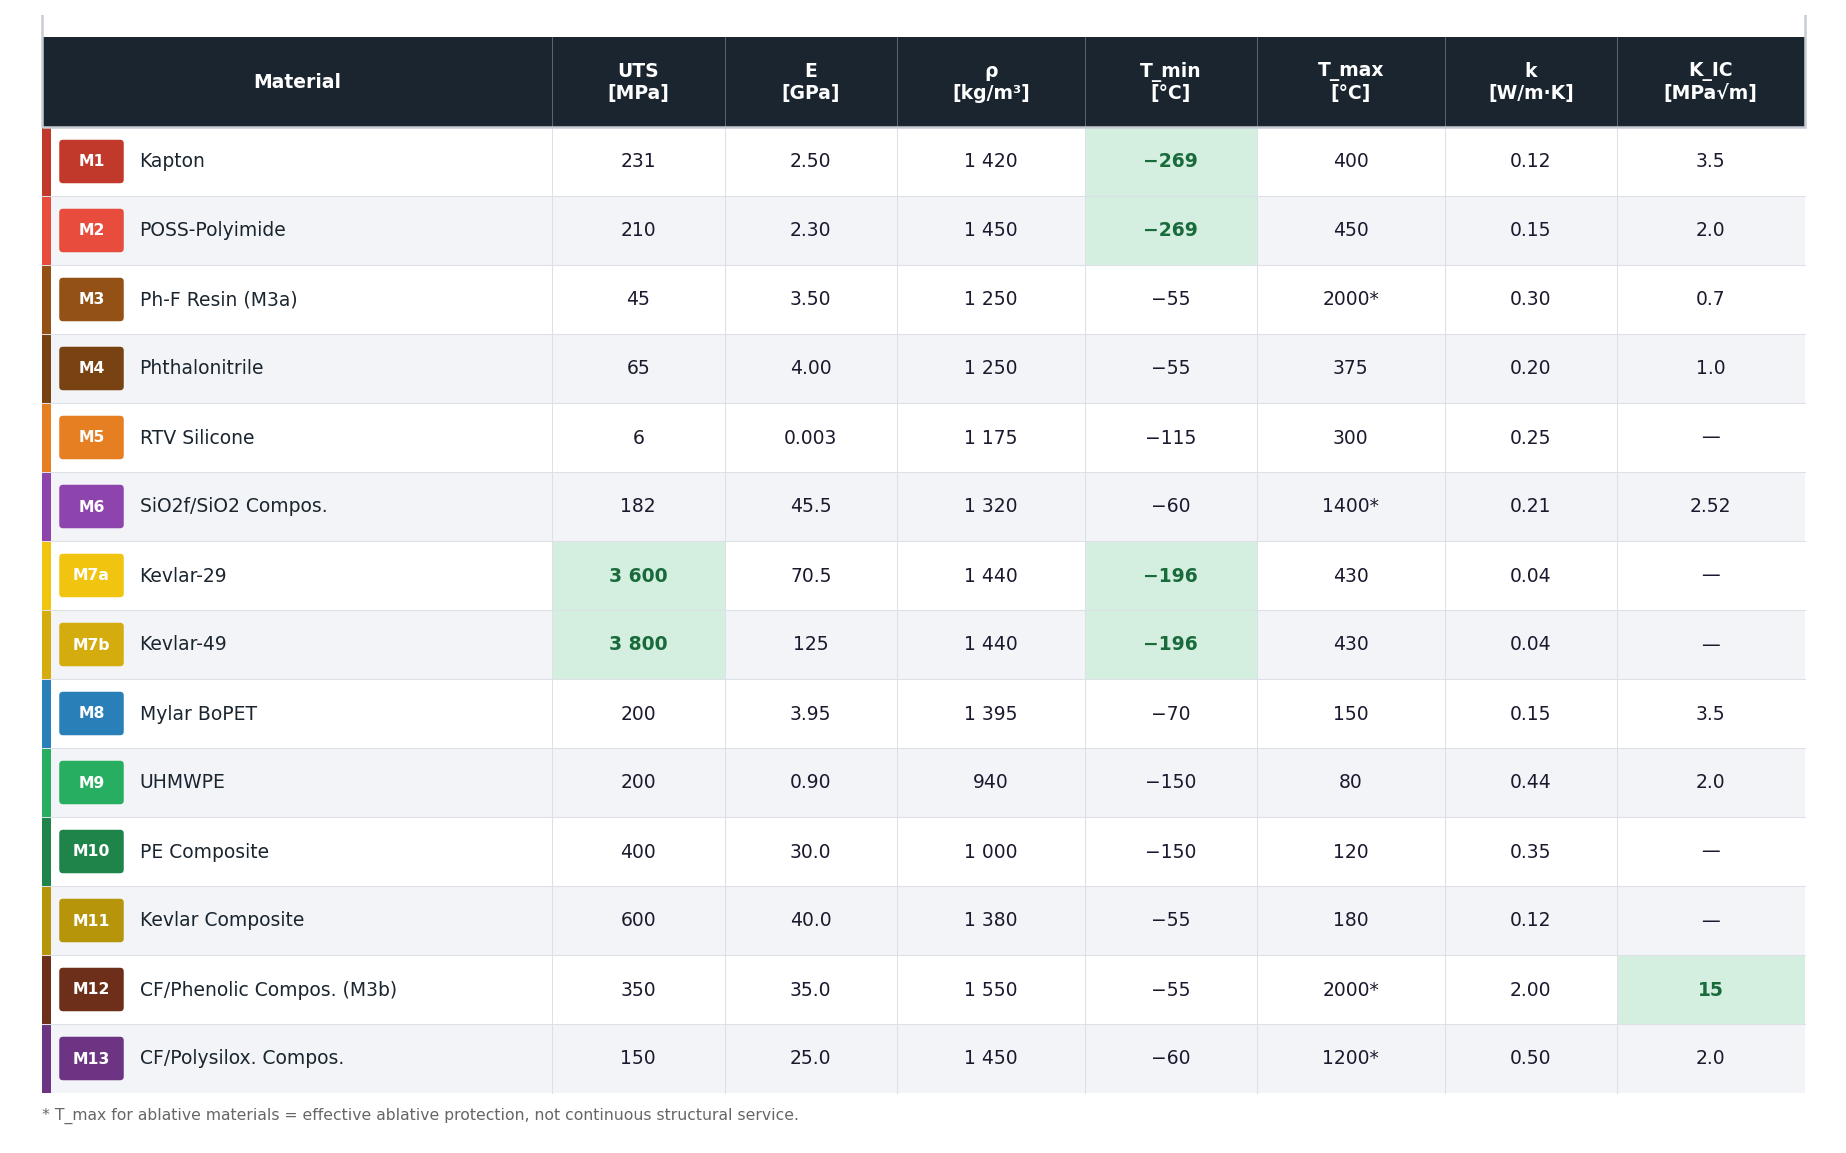
\includegraphics[width=\linewidth]{compare_G_table.png}
  \caption{\textit{Room-temperature material properties for M1--M13.
    Green cells denote top-performance values: UTS\,$\geq$\,3000\,MPa,
    $T_{\mathrm{min}}$\,$\leq$\,$-$196\,°C, $K_{\mathrm{IC}}$\,$\geq$\,10\,MPa$\sqrt{\mathrm{m}}$.
    Asterisk denotes effective ablative service temperature, not continuous
    structural service.}}
  \label{fig:table_summary}
\end{figure}

\subsection*{Tensile Strength}

The UTS comparison in Figure~\ref{fig:uts} is plotted on a logarithmic scale
because the data span four decades. Kevlar fibres (M7a, M7b) are dominant at
3600--3800\,MPa — more than six times the UTS of the next structural composite
(Kevlar/epoxy M11, 600\,MPa). At the lower end, the neat thermoset resins M3
and M4 record 45--65\,MPa, and the RTV elastomer M5 only 6\,MPa.

\begin{figure}[h!]
  \centering
  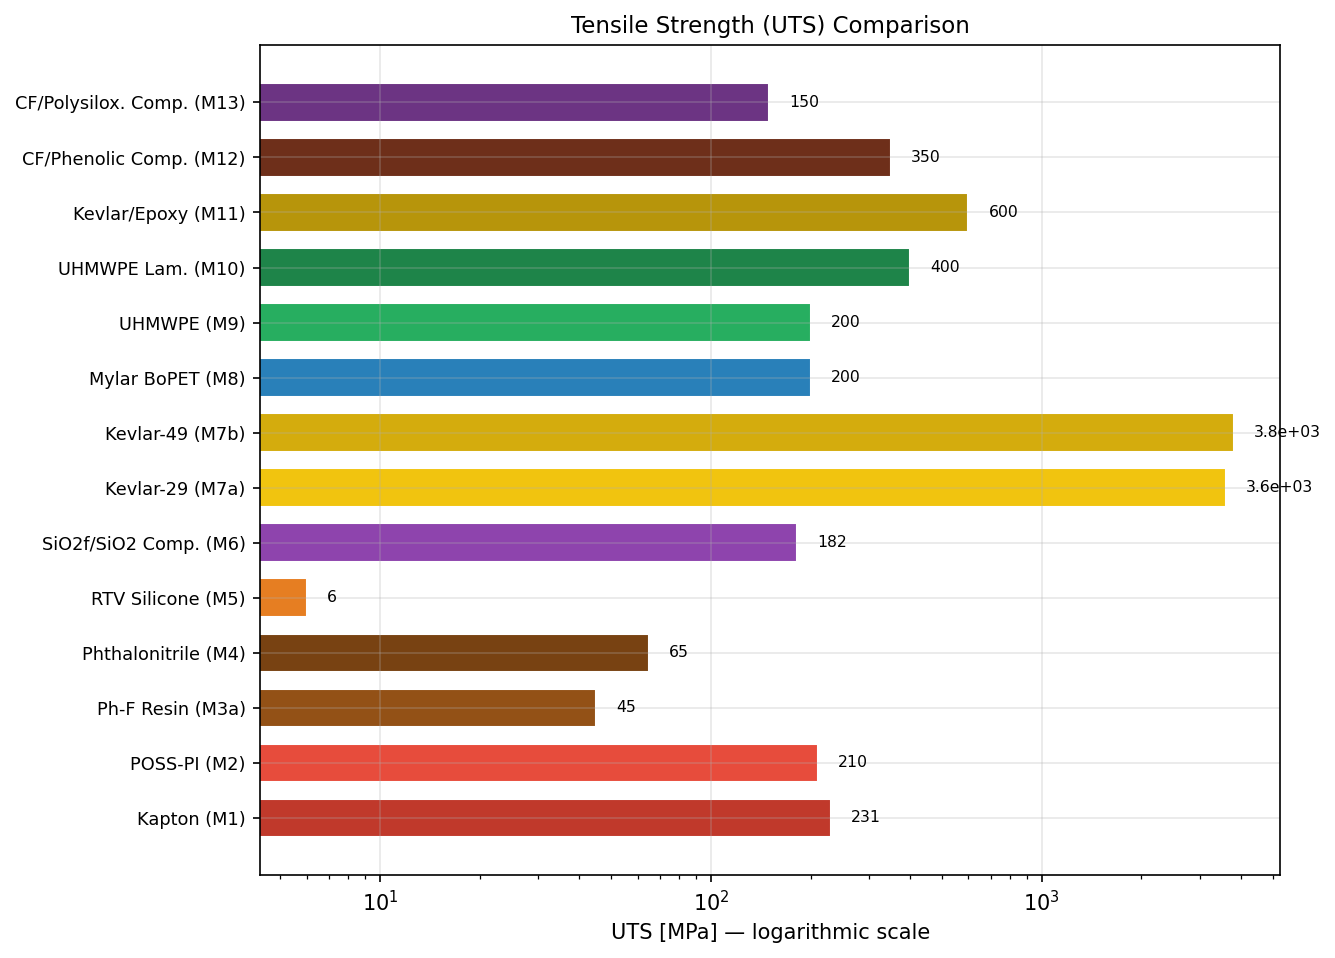
\includegraphics[width=\linewidth]{compare_A_uts.png}
  \caption{\textit{Tensile strength (UTS) comparison of M1--M13, logarithmic scale.}}
  \label{fig:uts}
\end{figure}

\subsection*{Young's Modulus and Stiffness}

The stiffness hierarchy (Figure~\ref{fig:modulus}) follows a similar pattern.
Kevlar-49 (M7b, 125\,GPa) is the stiffest organic material known, approaching
the modulus of aluminium alloys at one-third the density. SiO$_{2}$f/SiO$_{2}$ polysiloxane composite
(M6, 45.5\,GPa) and Kevlar/epoxy (M11, 40\,GPa) represent practical laminate
options when stiffness-to-weight ratio governs the design. RTV silicone (M5,
0.003\,GPa) is six orders of magnitude more compliant — its role is vibration
damping and sealing, not structural load bearing.

\begin{figure}[h!]
  \centering
  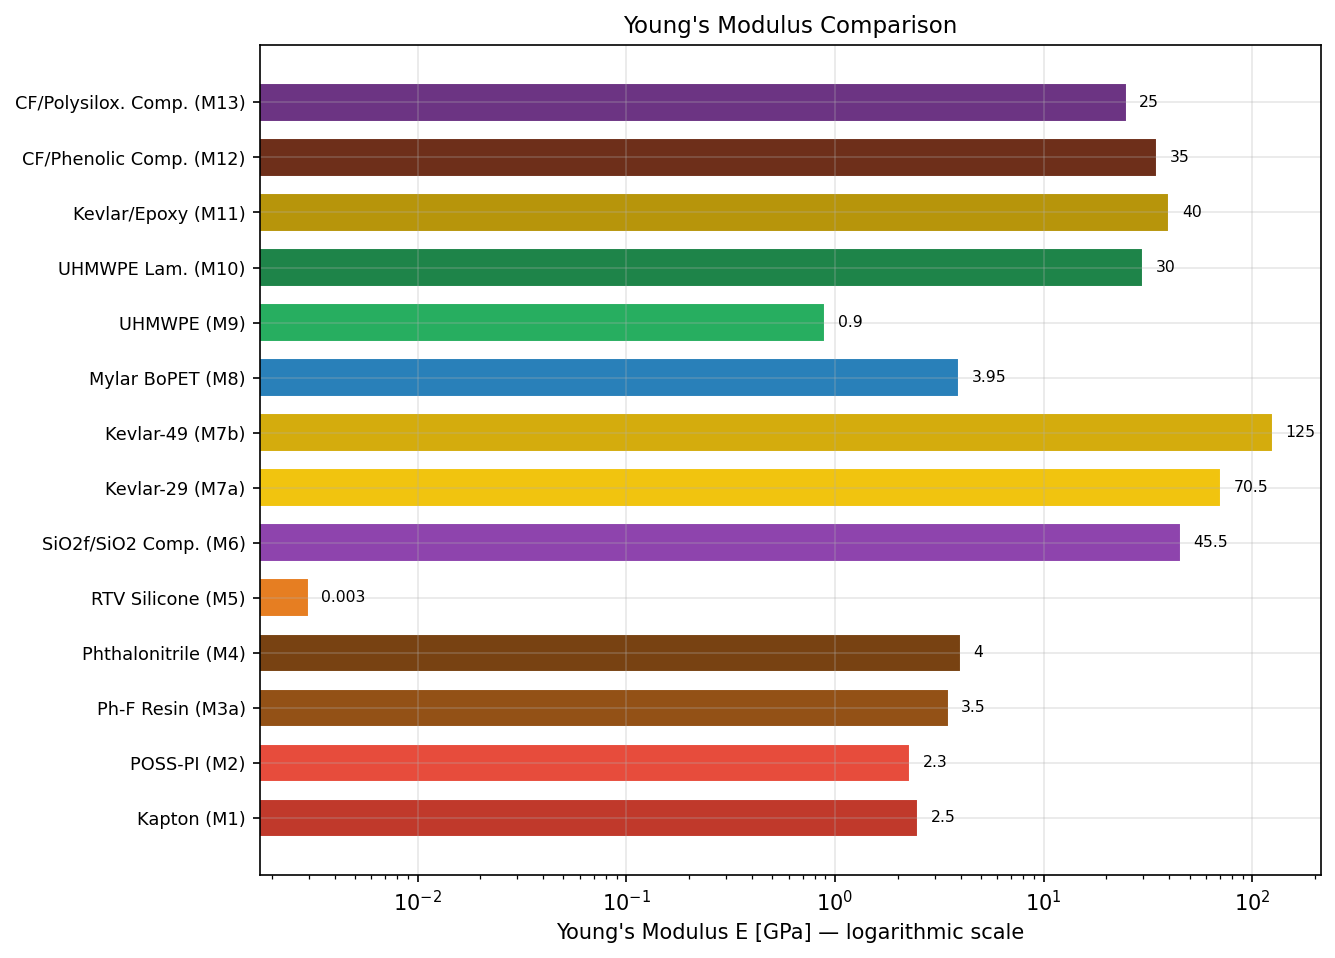
\includegraphics[width=\linewidth]{compare_B_modulus.png}
  \caption{\textit{Young's modulus comparison of M1--M13, logarithmic scale.}}
  \label{fig:modulus}
\end{figure}

\subsection*{Density and Specific Strength}

Figure~\ref{fig:density} shows densities ranging from 940\,kg/m$^{3}$ (UHMWPE, M9)
to 1550\,kg/m$^{3}$ (carbon/phenolic composite, M12). The narrow density range is a
characteristic of organic materials and contrasts sharply with metals
(2700--8900\,kg/m$^{3}$).

\begin{figure}[h!]
  \centering
  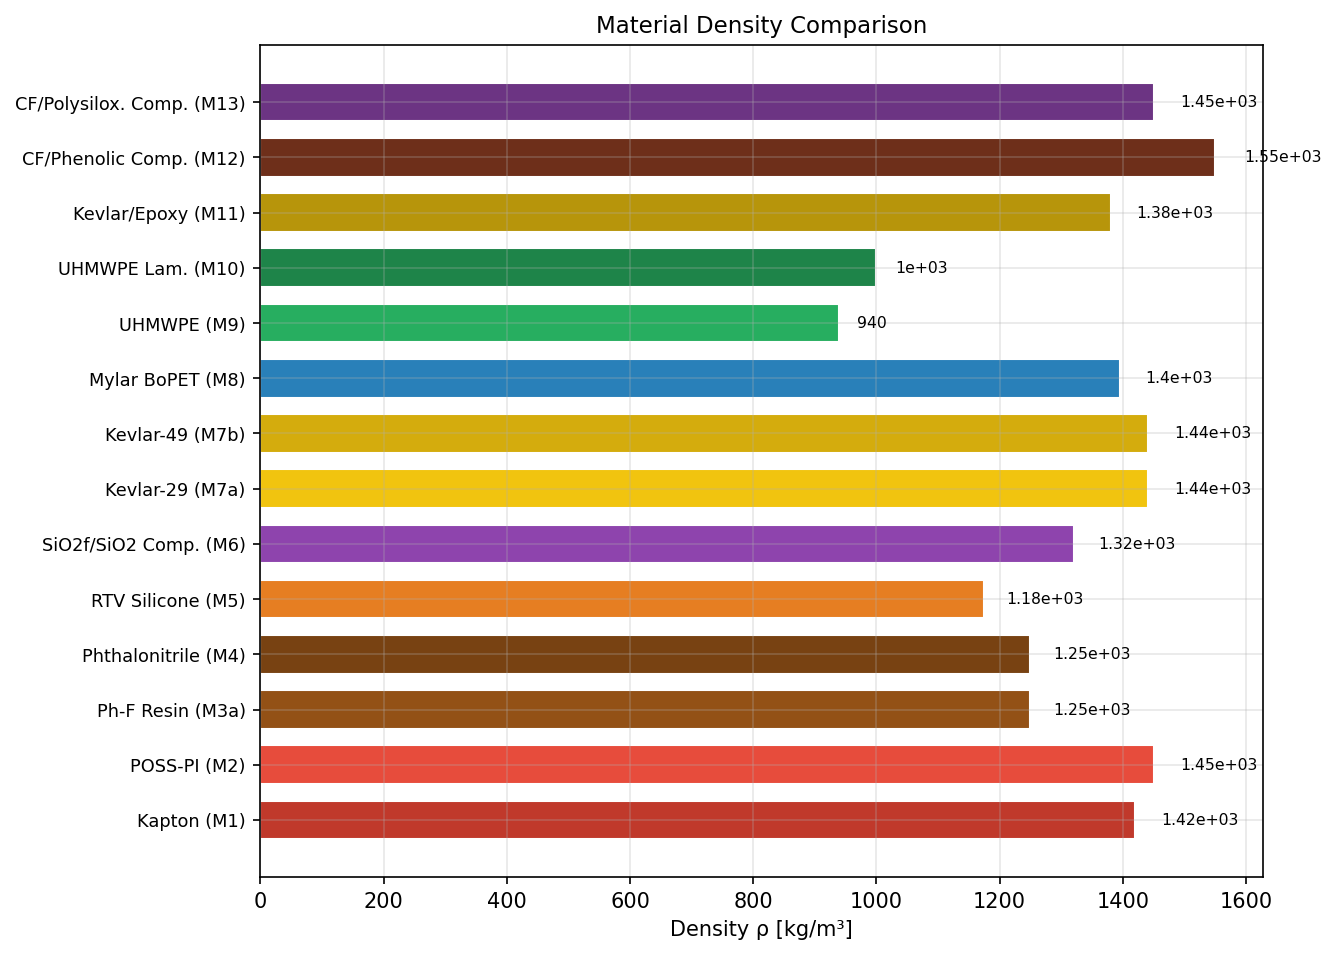
\includegraphics[width=\linewidth]{compare_C_density.png}
  \caption{\textit{Density comparison of M1--M13.
    UHMWPE (M9) is the only material with density below that of water.}}
  \label{fig:density}
\end{figure}

Specific strength (Figure~\ref{fig:specstrength}) reveals the true competitive
advantage of Kevlar: at 2.5\,km$^{2}$/s$^{2}$, it exceeds carbon-fibre/phenolic
composite (M12) by a factor of seven and polyimide film (M1) by a factor of
fifteen. For mass-critical structural applications, Kevlar fibres have no organic
competitor.

\begin{figure}[h!]
  \centering
  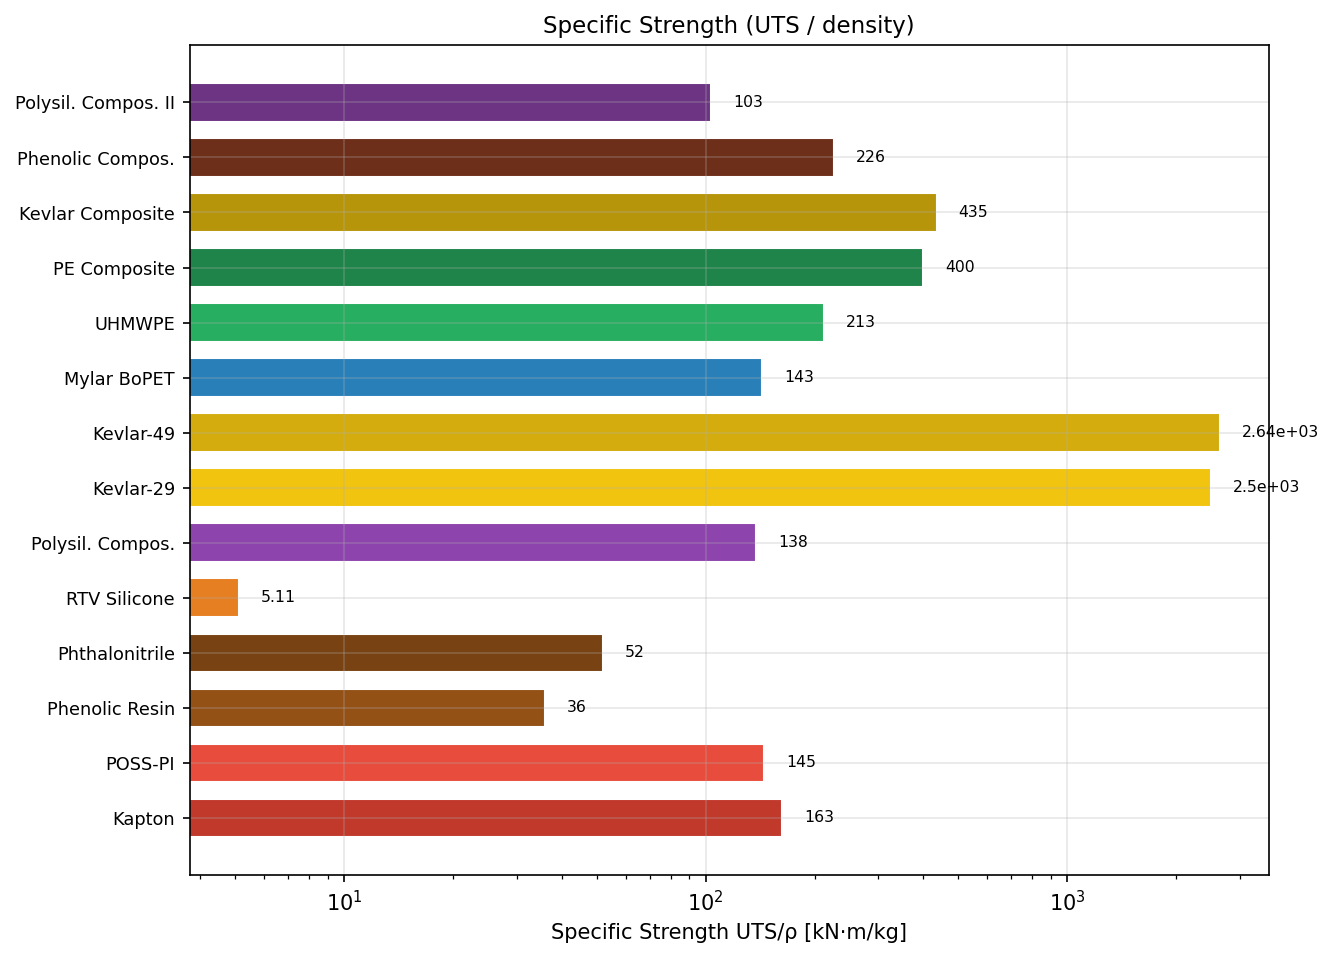
\includegraphics[width=\linewidth]{compare_E_spec_strength.png}
  \caption{\textit{Specific strength (UTS/$\rho$) comparison of M1--M13.}}
  \label{fig:specstrength}
\end{figure}

\subsection*{Service Temperature Range}

Figure~\ref{fig:temprange} presents service temperature ranges. Ablative
materials (M3, M6, M12, M13) cover the widest thermal envelopes, with effective
protection extending above 1000\,°C via char or SiOC-ceramic formation.
Kapton (M1) and POSS-PI (M2) cover the widest continuous service range
($-269$ to $+400/450\,^{\circ}$C), encompassing both the cryogenic propellant
temperature and the aerodynamic heating regime. The LEO thermal cycling envelope
of $-150$ to $+150\,^{\circ}$C is covered by all materials except UHMWPE
(limited to $+80\,^{\circ}$C), which is therefore unsuitable for external LEO
surfaces.

\begin{figure}[h!]
  \centering
  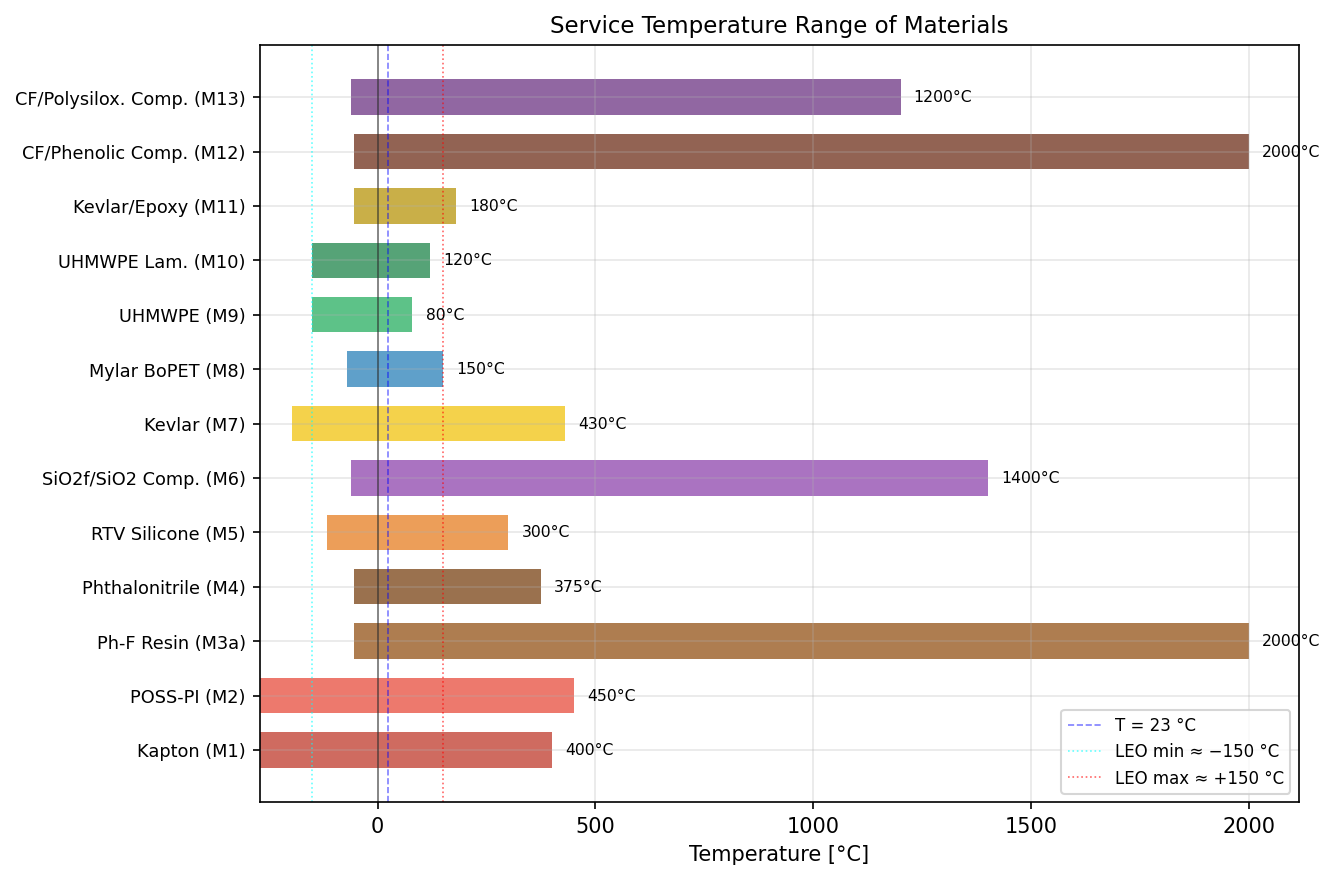
\includegraphics[width=\linewidth]{compare_D_temp_range.png}
  \caption{\textit{Service temperature range of M1--M13.
    Dotted lines mark the LEO thermal envelope ($-150$ to $+150$\,°C).}}
  \label{fig:temprange}
\end{figure}

% ────────────────────────────────────────────────────────────
%  5. MATERIAL SELECTION
% ────────────────────────────────────────────────────────────
\section*{Material Selection for Spacecraft Applications}

\subsection*{Scoring Methodology}

Five criteria are used to score each material for combined launch-phase and
LEO service. Weights reflect the relative severity of each threat in a typical
LEO mission:

\begin{itemize}[leftmargin=0.63cm, topsep=0pt, itemsep=0pt, parsep=0pt]
  \item Specific strength UTS/$\rho$ \dotfill 25\%
  \item Service temperature range $T_{\mathrm{max}} - T_{\mathrm{min}}$ \dotfill 20\%
  \item Resistance to atomic oxygen and UV radiation \dotfill 20\%
  \item Heat absorption / ablative capacity \dotfill 20\%
  \item Fracture toughness $K_{\mathrm{IC}}$ / impact resistance \dotfill 15\%
\end{itemize}

Each criterion is normalised to the interval $[0, 1]$ across all thirteen
materials and multiplied by the criterion weight. The resulting scores are
visualised in the radar chart (Figure~\ref{fig:radar}).

\begin{figure}[h!]
  \centering
  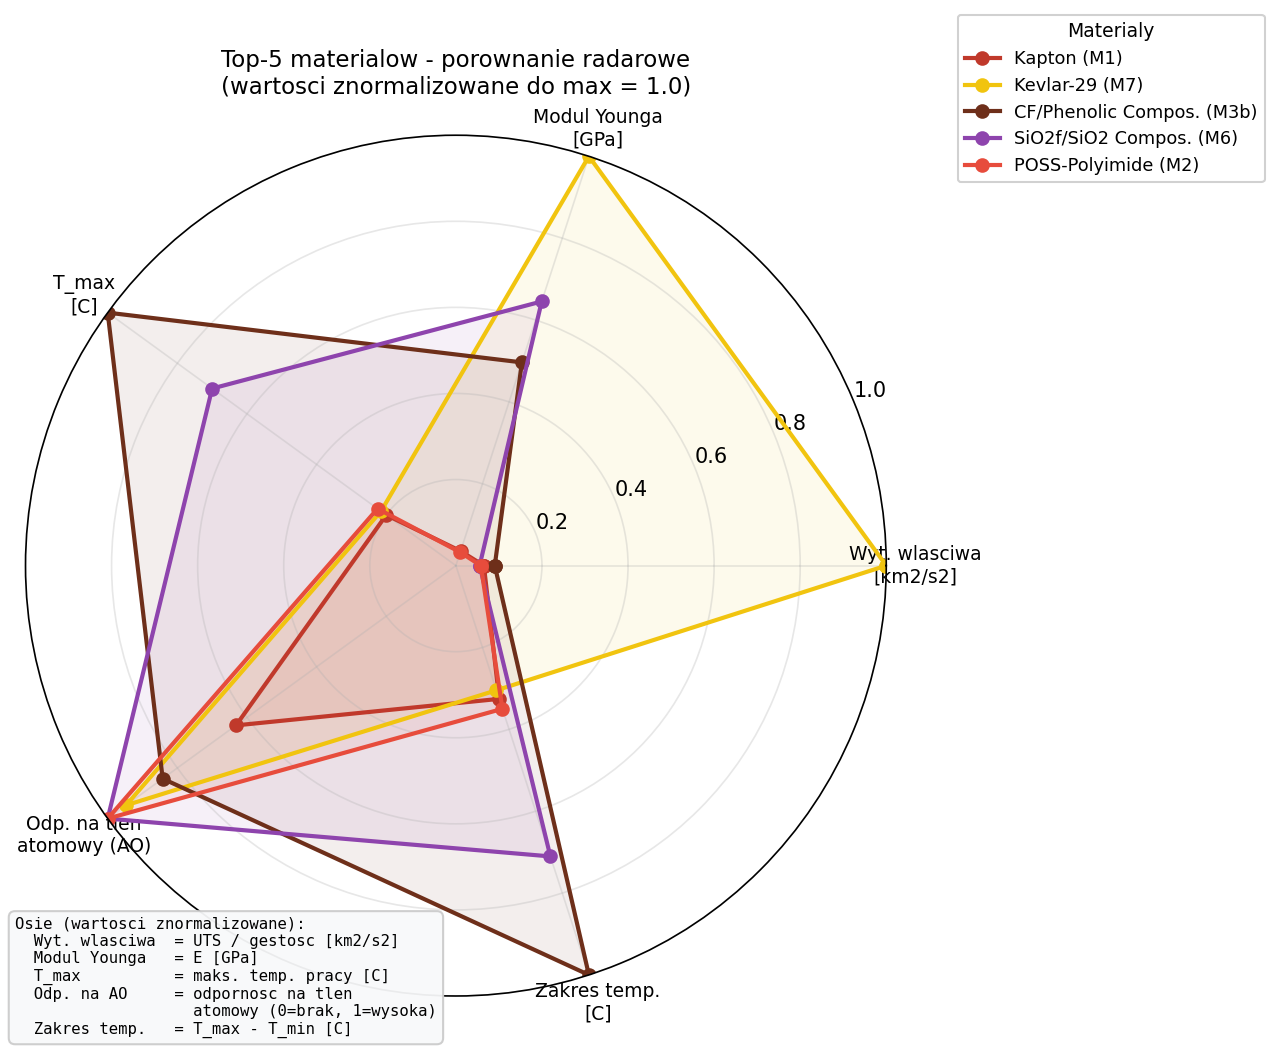
\includegraphics[width=0.80\linewidth]{compare_F_radar_top5.png}
  \caption{\textit{Multi-criteria radar comparison of the Top-5 candidate
    materials (normalised values, $\mathrm{max} = 1.0$).}}
  \label{fig:radar}
\end{figure}

\subsection*{Top-5 Recommended Materials}

A LEO spacecraft hull protection system must perform across two fundamentally
different mission phases: the \textbf{launch phase} (aerodynamic heating up to
several MW/m$^{2}$, intense acoustic loading during max-Q, and mechanical shock
at stage separation) and the \textbf{on-orbit phase} (continuous thermal cycling
between $-150$ and $+150\,^{\circ}$C, atomic oxygen erosion at fluences exceeding
$10^{20}$\,atoms/cm$^{2}$/year, UV/VUV radiation, and hypervelocity MMOD impacts).
The five recommended materials address these phases in complementary roles within
a multi-layer protection architecture.

\subsubsection*{1. Kapton HN (M1) — Primary LEO Surface Film}

Kapton is the universal outer-surface material for the on-orbit phase. Its
service range of $-269$ to $+400\,^{\circ}$C covers the full LEO thermal cycling
envelope with margin, vacuum outgassing is effectively zero, and 60 years of
flight heritage span every class of spacecraft from CubeSats to planetary probes.
During launch, Kapton MLI blankets are protected inside the payload fairing and
are therefore not exposed to aerodynamic heating. The AO erosion rate of
$3\,\times\,10^{-24}$\,cm$^{3}$/atom is well-characterised and managed by
vapour-deposited SiO$_{2}$ or Al$_{2}$O$_{3}$ overcoats (DuPont 2023).

\subsubsection*{2. Kevlar-29/49 (M7) — MMOD Shield and Structural Layer}

Kevlar's specific strength of 2.5\,km$^{2}$/s$^{2}$ and exceptional energy
absorption during hypervelocity impact — via progressive fibre pull-out and
fracture — make it the baseline material for Whipple and multi-shock shields
throughout the on-orbit phase. During launch it serves as the primary structural
fibre in pressure vessels (propellant tanks, pressurant bottles) and in
load-bearing interstage elements subjected to max-Q dynamic pressure. Temperature
stability from $-196$ to $+430\,^{\circ}$C covers both cryogenic propellant
contact and aerodynamic heating of lightly shielded structural members (DuPont 2017).

\subsubsection*{3. SiO$_{2}$f/SiO$_{2}$ Polysiloxane Composite (M6) — Launch TPS with On-Orbit AO Passivation}

M6 addresses both mission phases simultaneously. During launch its ablative
SiOC ceramic matrix absorbs aerodynamic heat fluxes up to 1400\,°C through
controlled pyrolysis, protecting interstage sections and fairing attachment
rings exposed after separation. On orbit, the SiO$_{2}$-rich surface formed
during ablation acts as a self-renewing passive barrier against atomic oxygen,
eliminating the need for a separate AO-protective coating on those surfaces.
Structural properties (UTS = 182\,MPa, $E$ = 45.5\,GPa) allow M6 to carry
moderate mechanical loads without a separate load-bearing substructure
(McDermott et al.\ 2022).

\subsubsection*{4. Carbon-Fibre/Phenolic Composite (M12) — Primary Launch-Phase TPS}

M12 is the first-choice material for surfaces experiencing the most severe
thermal loads during ascent: nozzle liners, rocket-motor interstage insulation,
and heat shield panels protecting avionics bays during max-Q. Heat fluxes of
several MW/m$^{2}$ drive char formation above 300\,°C; the resulting carbon
layer is thermally stable beyond 2000\,°C and structurally reinforced by carbon
fibres ($K_{\mathrm{IC}}$ = 15\,MPa$\,\mathrm{m}^{0.5}$), preventing
catastrophic cracking under acoustic and thermal shock. High in-plane thermal
conductivity ($k$ = 2.0\,W/(m$\cdot$K)) redistributes heat laterally, reducing
peak temperatures at attachment points (Tran et al.\ 2014, p.\,1418; Natali
et al.\ 2012, p.\,180).

\subsubsection*{5. POSS-Polyimide (M2) — Long-Duration LEO Surface Film}

Where mission duration exceeds five years or orbital altitude raises the AO
fluence above $10^{21}$\,atoms/cm$^{2}$, Kapton's erosion rate becomes
mission-limiting. POSS-PI replaces or supplements Kapton on the highest-priority
external surfaces: the polyhedral oligomeric silsesquioxane cages incorporated
into the polyimide backbone convert under AO attack to a continuous SiO$_{2}$
passivation layer in-situ, without requiring a pre-applied coating. Upper service
temperature of $+450\,^{\circ}$C provides an additional $50\,^{\circ}$C margin
over Kapton during post-separation transient heating (Brunsvold et al.\ 2004,
p.\,303; Gouzman et al.\ 2010, p.\,2440).

% ────────────────────────────────────────────────────────────
%  6. CONCLUSIONS
% ────────────────────────────────────────────────────────────
\specialsection{Conclusions}

A systematic comparison of thirteen organic materials for LEO spacecraft hull
protection has been conducted, evaluated across the two critical mission phases:
launch ascent and on-orbit operation. The principal findings are:

\begin{enumerate}[leftmargin=0.63cm, topsep=0pt, itemsep=0pt, parsep=0pt]
  \item No single material satisfies all hull-protection requirements across both
    mission phases. A multi-layer architecture is necessary: an outer surface film
    (M1 or M2) for on-orbit AO/UV/thermal control, a MMOD Whipple shield layer
    (M7), and a launch-phase TPS layer (M12 or M6) on thermally exposed surfaces.
  \item Ablative composites (M6, M12) are indispensable for the launch phase.
    Carbon-fibre/phenolic (M12) handles peak heat fluxes at nozzles and interstage
    sections; SiO$_{2}$f/SiO$_{2}$ polysiloxane (M6) provides ablative protection
    at moderate fluxes while its post-ablation SiO$_{2}$ surface doubles as an
    on-orbit AO barrier.
  \item Kevlar fibres (M7) are the only materials in the set with specific strength
    exceeding 2.0\,km$^{2}$/s$^{2}$ and cover both phases: MMOD shielding on orbit
    and structural pressure vessels during launch.
  \item Polyimide films (M1, M2) are the standard on-orbit external surface material.
    POSS-PI (M2) is preferred for missions longer than five years or at high AO
    fluence orbits; Kapton (M1) remains the cost-effective baseline for shorter
    missions.
  \item UHMWPE-based materials (M9, M10), despite attractive ballistic performance,
    are disqualified from external hull roles by their melt temperature
    ($\leq$\,135\,°C) — incompatible with launch aerodynamic heating — and by AO
    susceptibility on orbit.
\end{enumerate}

% ────────────────────────────────────────────────────────────
%  APPENDIX — FULL PROPERTY DATA TABLE
% ────────────────────────────────────────────────────────────
\specialsection{Appendix: Complete Property Data with Sources}

{\fontsize{8}{9.5}\selectfont
\setlength{\LTpre}{4pt}
\setlength{\LTpost}{4pt}
\begin{longtable}{@{} p{2.5cm} p{2.7cm} p{1.6cm} p{1.0cm} p{5.0cm} @{}}
\caption{\textit{Complete room-temperature (23\,°C) mechanical and thermal
  properties of M1--M13 with primary source and page reference.
  Asterisk (*) on T\textsubscript{max} denotes effective ablative
  service temperature, not continuous structural limit.
  ``est.'' = value estimated from related data in cited source.}}
\label{tab:fulldata} \\
\toprule
\textbf{Material} & \textbf{Property} & \textbf{Value} & \textbf{Unit}
  & \textbf{Source} \\
\midrule
\endfirsthead
\multicolumn{5}{l}{\footnotesize\itshape (Table~\ref{tab:fulldata} continued)} \\
\toprule
\textbf{Material} & \textbf{Property} & \textbf{Value} & \textbf{Unit}
  & \textbf{Source} \\
\midrule
\endhead
\midrule
\multicolumn{5}{r}{\footnotesize\itshape Continued on next page\ldots} \\
\endfoot
\bottomrule
\endlastfoot

%% ── M1 Kapton ───────────────────────────────────────────────
\multirow{6}{2.5cm}{\textbf{M1}\\Kapton HN\\(DuPont)}
  & UTS              & 231        & MPa        & DuPont (2023), datasheet p.~1 \\
  & Young's mod.\ $E$& 2.5        & GPa        & DuPont (2023), datasheet p.~1 \\
  & Density $\rho$   & 1\,420     & kg/m$^3$   & DuPont (2023), datasheet p.~1 \\
  & Therm.\ cond.\ $k$ & 0.12     & W/m$\cdot$K & DuPont (2023), datasheet p.~2 \\
  & T range          & $-$269\,/\,$+$400 & °C  & DuPont (2023), datasheet p.~1 \\
  & $K_\mathrm{IC}$  & 1.65--5.4  & MPa$\sqrt{\text{m}}$ & DuPont (2023), datasheet p.~2 \\
\midrule

%% ── M2 POSS-PI ──────────────────────────────────────────────
\multirow{6}{2.5cm}{\textbf{M2}\\POSS-Poly\-imide}
  & UTS              & 210        & MPa        & Brunsvold et al.\ (2004), p.~303 \\
  & Young's mod.\ $E$& 2.3        & GPa        & Brunsvold et al.\ (2004), p.~303 \\
  & Density $\rho$   & 1\,450     & kg/m$^3$   & Brunsvold et al.\ (2004), p.~303 \\
  & Therm.\ cond.\ $k$ & 0.15     & W/m$\cdot$K & Gouzman et al.\ (2010), p.~2440 \\
  & T range          & $-$269\,/\,$+$450 & °C  & Gouzman et al.\ (2010), p.~2439 \\
  & $K_\mathrm{IC}$  & $\approx$2.0 & MPa$\sqrt{\text{m}}$ & Gouzman et al.\ (2010), p.~2440 (est.) \\
\midrule

%% ── M3a Ph-F Resin ──────────────────────────────────────────
\multirow{6}{2.5cm}{\textbf{M3a}\\Ph-F Resin\\(SC-1008)}
  & UTS              & 45         & MPa        & AZoM ID:475 \\
  & Young's mod.\ $E$& 3.5        & GPa        & AZoM ID:475 \\
  & Density $\rho$   & 1\,250     & kg/m$^3$   & AZoM ID:475 \\
  & Therm.\ cond.\ $k$ & 0.30     & W/m$\cdot$K & AZoM ID:475 \\
  & T range          & $-$55\,/\,$>$2000* & °C & Natali et al.\ (2012), p.~3 \\
  & $K_\mathrm{IC}$  & 0.7        & MPa$\sqrt{\text{m}}$ & AZoM ID:475 \\
\midrule

%% ── M4 Phthalonitrile ───────────────────────────────────────
\multirow{6}{2.5cm}{\textbf{M4}\\Phthalo-nitrile Resin}
  & UTS              & 65         & MPa        & Hergenrother et al.\ (2005), p.~7853 \\
  & Young's mod.\ $E$& 4.0        & GPa        & Hergenrother et al.\ (2005), p.~7853 \\
  & Density $\rho$   & 1\,250     & kg/m$^3$   & Hergenrother et al.\ (2005), p.~7853 \\
  & Therm.\ cond.\ $k$ & 0.20     & W/m$\cdot$K & Hergenrother et al.\ (2005), p.~7853 \\
  & T range          & $-$55\,/\,$+$375  & °C  & Hergenrother et al.\ (2005), p.~7851 \\
  & $K_\mathrm{IC}$  & 1.0        & MPa$\sqrt{\text{m}}$ & Laskoski et al.\ (2006), p.~4559 \\
\midrule

%% ── M5 RTV Silicone ─────────────────────────────────────────
\multirow{5}{2.5cm}{\textbf{M5}\\RTV Silicone\\(Momentive RTV566)}
  & UTS              & 6          & MPa        & AZoM ID:920; MatWeb RTV566 \\
  & Young's mod.\ $E$& 0.003      & GPa        & AZoM ID:920 \\
  & Density $\rho$   & 1\,175     & kg/m$^3$   & AZoM ID:920; MatWeb RTV566 \\
  & Therm.\ cond.\ $k$ & 0.25     & W/m$\cdot$K & AZoM ID:920 \\
  & T range          & $-$115\,/\,$+$300 & °C  & Barucci et al.\ (1998), p.~3 \\
\midrule

%% ── M6 SiO2f/SiO2 ───────────────────────────────────────────
\multirow{6}{2.5cm}{\textbf{M6}\\SiO$_2$f/SiO$_2$\\Polysilox.}
  & UTS              & 182        & MPa        & McDermott et al.\ (2022), p.~3207 \\
  & Young's mod.\ $E$& 45.5       & GPa        & Hou et al.\ (Techneglas, 2021) \\
  & Density $\rho$   & 1\,320     & kg/m$^3$   & McDermott et al.\ (2022), p.~3204 \\
  & Therm.\ cond.\ $k$ & 0.21     & W/m$\cdot$K & McDermott et al.\ (2022), p.~3210 \\
  & T range          & $-$60\,/\,$+$1400* & °C & Hou et al.\ (Techneglas, 2021) \\
  & $K_\mathrm{IC}$  & 2.52       & MPa$\sqrt{\text{m}}$ & PMC11945185 (2025) \\
\midrule

%% ── M7a Kevlar-29 ───────────────────────────────────────────
\multirow{5}{2.5cm}{\textbf{M7a}\\Kevlar-29\\(DuPont)}
  & UTS              & 3\,600     & MPa        & DuPont (2017), Tech.\ Guide p.~5 \\
  & Young's mod.\ $E$& 70.5       & GPa        & DuPont (2017), Tech.\ Guide p.~5 \\
  & Density $\rho$   & 1\,440     & kg/m$^3$   & DuPont (2017), Tech.\ Guide p.~4 \\
  & Therm.\ cond.\ $k$ & 0.04     & W/m$\cdot$K & Ventura \& Martelli (2009), p.~735 \\
  & T range          & $-$196\,/\,$+$430 & °C  & DuPont (2017), Tech.\ Guide p.~6 \\
\midrule

%% ── M7b Kevlar-49 ───────────────────────────────────────────
\multirow{5}{2.5cm}{\textbf{M7b}\\Kevlar-49\\(DuPont)}
  & UTS              & 3\,800     & MPa        & DuPont (2017), Tech.\ Guide p.~5 \\
  & Young's mod.\ $E$& 125        & GPa        & DuPont (2017), Tech.\ Guide p.~5 \\
  & Density $\rho$   & 1\,440     & kg/m$^3$   & DuPont (2017), Tech.\ Guide p.~4 \\
  & Therm.\ cond.\ $k$ & 0.04     & W/m$\cdot$K & Ventura \& Martelli (2009), p.~735 \\
  & T range          & $-$196\,/\,$+$430 & °C  & DuPont (2017), Tech.\ Guide p.~6 \\
\midrule

%% ── M8 Mylar BoPET ──────────────────────────────────────────
\multirow{6}{2.5cm}{\textbf{M8}\\Mylar BoPET\\(DuPont Teijin)}
  & UTS              & 200        & MPa        & DuPont Teijin (2021), datasheet p.~1 \\
  & Young's mod.\ $E$& 3.95       & GPa        & DuPont Teijin (2021), datasheet p.~1 \\
  & Density $\rho$   & 1\,395     & kg/m$^3$   & DuPont Teijin (2021), datasheet p.~1 \\
  & Therm.\ cond.\ $k$ & 0.15     & W/m$\cdot$K & DuPont Teijin (2021), datasheet p.~2 \\
  & T range          & $-$70\,/\,$+$150  & °C  & DuPont Teijin (2021), datasheet p.~2 \\
  & $K_\mathrm{IC}$  & $\approx$3.5 & MPa$\sqrt{\text{m}}$ & AZoM ID:2047 (est.) \\
\midrule

%% ── M9 UHMWPE ───────────────────────────────────────────────
\multirow{6}{2.5cm}{\textbf{M9}\\UHMWPE\\(bulk)}
  & UTS              & 200        & MPa        & Kurtz (2009), ch.~2, p.~23 \\
  & Young's mod.\ $E$& 0.9        & GPa        & Sobieraj \& Rimnac (2009), p.~433 \\
  & Density $\rho$   & 940        & kg/m$^3$   & AZoM ID:1831 \\
  & Therm.\ cond.\ $k$ & 0.44     & W/m$\cdot$K & AZoM ID:1831 \\
  & T range          & $-$150\,/\,$+$80  & °C  & Kurtz (2009), ch.~2, p.~23 \\
  & $K_\mathrm{IC}$  & $\approx$2.0 & MPa$\sqrt{\text{m}}$ & Sobieraj \& Rimnac (2009), p.~433 \\
\midrule

%% ── M10 UHMWPE Laminate ─────────────────────────────────────
\multirow{5}{2.5cm}{\textbf{M10}\\UHMWPE Lam.\\(Dyneema SK75)}
  & UTS              & 400        & MPa        & Koh et al.\ (2010), p.~2234 \\
  & Young's mod.\ $E$& 30         & GPa        & Koh et al.\ (2010), p.~2236 \\
  & Density $\rho$   & 1\,000     & kg/m$^3$   & DSM Dyneema UD datasheet \\
  & Therm.\ cond.\ $k$ & 0.35     & W/m$\cdot$K & AZoM ID:1831 (est., composite rule) \\
  & T range          & $-$150\,/\,$+$120 & °C  & DSM Dyneema UD datasheet \\
\midrule

%% ── M11 Kevlar/Epoxy ────────────────────────────────────────
\multirow{5}{2.5cm}{\textbf{M11}\\Kevlar/Epoxy\\(Hexcel 8552)}
  & UTS              & 600        & MPa        & Duan et al.\ (2006), p.~441 \\
  & Young's mod.\ $E$& 40         & GPa        & DuPont Kevlar Design Guide \\
  & Density $\rho$   & 1\,380     & kg/m$^3$   & DuPont Kevlar Design Guide \\
  & Therm.\ cond.\ $k$ & 0.12     & W/m$\cdot$K & DuPont (2017), Tech.\ Guide p.~8 \\
  & T range          & $-$55\,/\,$+$180  & °C  & Hexcel 8552 epoxy datasheet \\
\midrule

%% ── M12 CF/Phenolic ─────────────────────────────────────────
\multirow{6}{2.5cm}{\textbf{M12}\\CF/Phenolic\\Composite}
  & UTS              & 350        & MPa        & Natali et al.\ (2012), p.~5 \\
  & Young's mod.\ $E$& 35         & GPa        & Natali et al.\ (2012), p.~5 \\
  & Density $\rho$   & 1\,550     & kg/m$^3$   & Natali et al.\ (2012), p.~5 \\
  & Therm.\ cond.\ $k$ & 2.0      & W/m$\cdot$K & Tran et al.\ (2014), p.~1418 \\
  & T range          & $-$55\,/\,$>$2000* & °C & Natali et al.\ (2012), p.~5 \\
  & $K_\mathrm{IC}$  & 15         & MPa$\sqrt{\text{m}}$ & Tran et al.\ (2014), p.~1418 \\
\midrule

%% ── M13 CF/Polysiloxane ─────────────────────────────────────
\multirow{6}{2.5cm}{\textbf{M13}\\CF/Polysilox.\\Composite}
  & UTS              & 150        & MPa        & McDermott et al.\ (2022), p.~3209 \\
  & Young's mod.\ $E$& 25         & GPa        & McDermott et al.\ (2022), p.~3209 \\
  & Density $\rho$   & 1\,450     & kg/m$^3$   & McDermott et al.\ (2022), p.~3204 \\
  & Therm.\ cond.\ $k$ & 0.50     & W/m$\cdot$K & McDermott et al.\ (2022), p.~3210 \\
  & T range          & $-$60\,/\,$+$1200* & °C & Hou et al.\ (Techneglas, 2021) \\
  & $K_\mathrm{IC}$  & $\approx$2.0 & MPa$\sqrt{\text{m}}$ & PMC11945185 (2025) \\

\end{longtable}
}

% ────────────────────────────────────────────────────────────
%  REFERENCES
% ────────────────────────────────────────────────────────────
\specialsection{References}

{\fontsize{9.5}{11.4}\selectfont
\begin{enumerate}[label=\arabic*., leftmargin=1.5cm, topsep=0pt,
                  itemsep=0pt, parsep=0pt]

  \item Barucci M., Bianchini G., Gottardi E.\ et al.\ (1998), \textit{Low
    Temperature Thermal Properties of Some Filled Silicone Rubbers},
    ``Cryogenics'', 38, 5, pp.\ 3--6. DOI:~10.1016/S0011-2275(97)00111-3

  \item Brunsvold A.L., Minton T.K., Gouzman I.\ et al.\ (2004), \textit{An
    Investigation of the Resistance of POSS Polyimide to Atomic Oxygen Attack},
    ``High Performance Polymers'', 16, 2, pp.\ 303--318.
    DOI:~10.1177/0954008304024680

  \item Duan Y., Keefe M., Bogetti T.A.\ et al.\ (2006), \textit{Modeling the
    Role of Friction in the Ballistic Performance of a Plain-Weave Kevlar KM2
    Fabric}, ``International Journal of Impact Engineering'', 32, pp.\ 441--467.
    DOI:~10.1016/j.ijimpeng.2005.07.007

  \item DuPont (2017), \textit{Kevlar Technical Guide}, \url{https://www.dupont.com}
    (accessed: 05.05.2026)

  \item DuPont (2023), \textit{Kapton HN — General Specifications Datasheet},
    \url{https://www.dupont.com} (accessed: 05.05.2026)

  \item DuPont Teijin Films (2021), \textit{Mylar A Polyester Film — Datasheet},
    \url{https://www.dupont.com} (accessed: 05.05.2026)

  \item Gouzman I., Grossman E., Verker R.\ et al.\ (2010), \textit{Advances in
    Polyimide-Based Materials for Space Applications}, ``Advanced Materials'',
    22, pp.\ 2436--2445. DOI:~10.1002/adma.200903503

  \item Hergenrother P.M., Smith J.G., Connell J.W.\ et al.\ (2005),
    \textit{Phthalonitrile Resin for High-Temperature Polymer Matrix Composites},
    ``Polymer'', 46, pp.\ 7851--7861. DOI:~10.1016/j.polymer.2005.09.039

  \item Koh C.P., Shim V.P.W., Tan V.B.C.\ (2010), \textit{Response of a
    Reinforced UHMWPE Plate to Hypervelocity Impact}, ``International Journal of
    Impact Engineering'', 37, pp.\ 2234--2245. DOI:~10.1016/j.ijimpeng.2009.11.010

  \item Kurtz S.M.\ (ed.) (2009), \textit{UHMWPE Biomaterials Handbook}, 2nd ed.,
    Elsevier, Oxford. DOI:~10.1016/B978-0-12-374721-1.00002-7

  \item Laskoski M., Dominguez D.D., Keller T.M.\ (2006), \textit{Synthesis and
    Properties of a Liquid Phthalonitrile Resin}, ``Journal of Polymer Science
    Part A'', 44, pp.\ 4559--4565. DOI:~10.1002/pola.21358

  \item McDermott M.T., Rickard I., Grunenfelder L.K.\ (2022), \textit{High-Temperature
    Mechanical Behaviour of 2.5D~SiO$_{2}$/SiO$_{2}$ Composites}, ``Journal of
    Composite Materials'', 56, pp.\ 3201--3215. DOI:~10.1177/00219983211038622

  \item Natali M., Kenny J.M., Torre L.\ (2012), \textit{Science and Technology of
    Polymeric Ablative Materials for Thermal Protection Systems and Propulsion
    Devices}, ``Progress in Polymer Science'', 37, pp.\ 174--190.
    DOI:~10.1016/j.progpolymsci.2011.08.002

  \item Sobieraj M.C., Rimnac C.M.\ (2009), \textit{Ultra High Molecular Weight
    Polyethylene: Mechanics, Morphology, and Clinical Behaviour}, ``Journal of
    the Mechanical Behaviour of Biomedical Materials'', 2, pp.\ 433--443.
    DOI:~10.1016/j.jmbbm.2008.07.002

  \item Tran H., Johnson C., Rasky D.\ et al.\ (2014), \textit{Phenolic Impregnated
    Carbon Ablator (PICA) as Thermal Protection Systems for Discovery Missions},
    ``Journal of Spacecraft and Rockets'', 51, pp.\ 1418--1428.
    DOI:~10.2514/1.T4165

  \item Ventura G., Martelli V.\ (2009), \textit{Thermal Conductivity of Kevlar~49
    Between 7 and 290\,K}, ``Cryogenics'', 49, pp.\ 735--737.
    DOI:~10.1016/j.cryogenics.2009.04.001

\end{enumerate}
}

% ────────────────────────────────────────────────────────────
%  POLISH TITLE + STRESZCZENIE  (required for English-language texts)
% ────────────────────────────────────────────────────────────
\vspace{18pt}
\begin{center}
  {\cambriafont\fontsize{11}{13.2}\selectfont\bfseries
    Porównanie wybranych materiałów organicznych stosowanych\\
    jako poszycie kadłuba statku kosmicznego\\
    na niskiej orbicie okołoziemskiej\par}
\end{center}

\vspace{6pt}

\begingroup
  \setlength{\leftskip}{0.75cm}
  \setlength{\rightskip}{0.75cm}
  \fontsize{9}{10.8}\selectfont\noindent
  \textbf{Streszczenie:}
  Statki kosmiczne operujące na niskiej orbicie okołoziemskiej (LEO) oraz podczas
  startu narażone są na jednoczesne ekstremalne zagrożenia: erozję wywołaną
  atomowym tlenem (AO), promieniowanie ultrafioletowe, cykle termiczne w zakresie
  od $-150\,^{\circ}$C do $+150\,^{\circ}$C, uderzenia mikrometeorytów
  i szczątków orbitalnych, a podczas wznoszenia — strumienie ciepła
  1--10\,MW/m$^{2}$. Dobór materiałów poszycia i systemów ochrony termicznej
  wymaga kompromisu między niską gęstością powierzchniową, wytrzymałością
  mechaniczną, stabilnością termiczną i trwałością powierzchniową.
  W artykule przedstawiono systematyczne porównanie trzynastu materiałów
  organicznych (M1--M13) obejmujących folie poliimidowe, żywice termoutwardzalne,
  elastomery, włókna aramidowe oraz zaawansowane kompozyty. Właściwości
  mechaniczne i termiczne zestawiono na podstawie kart katalogowych producentów
  i recenzowanych publikacji naukowych. Wielokryterialna metoda oceny pozwoliła
  wyłonić pięć najlepszych materiałów: Kapton~HN (M1) i POSS-poliimid (M2) jako
  folie powierzchniowe LEO, Kevlar-29/49 (M7) do zastosowań strukturalnych
  i tarcz Whipple'a, kompozyt węglowo-fenolowy (M12) jako TPS wysokiego strumienia
  ciepła oraz kompozyt polisiloksanowy (M6) jako wielofunkcyjny materiał
  ablacyjno-strukturalny.
  \par\vspace{4pt}
  \noindent\textbf{Słowa kluczowe:}
  kompozyty organiczne, Kapton, Kevlar, materiały ablacyjne, niska orbita
  okołoziemska, poliimid, statek kosmiczny, system ochrony termicznej,
  tlen atomowy, włókna aramidowe
\endgroup

\end{document}
